%%%%%%%%%%%%%%%%%%%%%%%%%%%%%%%%%%%%%%%%%%%%%%%%%%%%%%%%%%%%%%%%%%%%%%%% NEED the picture attached inside the Sudoku.zip file to compile
%%%%%%%%%%%%%%%%%%%%%%%%%%%%%%%%%%%%%%%%%%%%%%%%%%%%%%%%%%%%%%%%%%%%%%%% Name of Picture SudokuSet.png
\documentclass[a4paper]{article}
\usepackage{a4wide}
\usepackage{longtable}
\usepackage{graphicx}
\usepackage{verbatim}
\usepackage{color}
\usepackage[normalem]{ulem}
%% gives strikeout capability with \sout{}
%Gummi|063|=)
\title{\textbf{Assignment 3 COMP2111 13s1\\Sudoku}}
\author{Jiashu Chen\\
}

\date{Revision 1.3 of Date: MAY/26/2013 19:20}


\begin{document}
\thispagestyle{empty}
\maketitle
\tableofcontents
\newpage
\setcounter{page}{1}

\section{Introduction}

\indent\indent The goal of the project is to develop a Sudoku solving assistant in Event-B.

The solver needs the following functionality.

\begin{description}
\item [Set up:] The event takes an incomplete grid and put it into the Sudoku Grid.
\item [Fill:] The event takes a position on the grid and a number, and fill it into the grid.
\item [Auto Fill:] When there is only one possibility of number for a grid cell, the number will be automatically filled into the grid.
\item [Hint:] Reveal a coordinate and it's possibility. (The cell with minimal possibility).
\item [Guess:] Fill the cell with one on the hinted number
\item [Alarm:] When the solver run into problem.
\item [Undo:] Remove number from a cell in the grid.
\end{description}

\vspace{1.5 cm}

\section{Problem Statement: Entity Representation and Requirements}

\subsection{Sudoku Representation}

\begin{figure}[h!]
  \begin{center}
  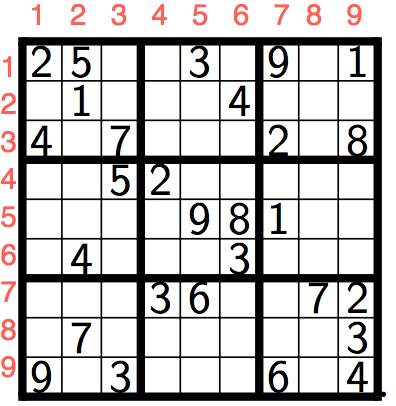
\includegraphics[width=0.35\textwidth]{SudokuSet.png}
  \caption{Sudoku Structure}
  \end{center}
\end{figure}


\noindent As shown in the diagram the structure representation of the traffic facilities around the hotel will be the following:\\
\newpage
\begin{longtable}{|l|p{2.4cm}|p{4.1cm}|p{4.5cm}|}
  \caption{Table of Hotel Traffic Entity Representation}\\
  \hline
  \multicolumn{1}{|c|}{\textbf{Type}}  &
  \multicolumn{1}{|c|}{\textbf{Name}} &
  \multicolumn{1}{|c|}{\textbf{Level First Introduced}} &
  \textbf{Short Description}\\
  \hline\hline
  \endfirsthead
  \caption[]{Table of Hotel Traffic Representation \textit{Continued}}\\
  \hline
  \multicolumn{1}{|c|}{\textbf{Type}}  &
  \multicolumn{1}{|c|}{\textbf{Name}} &
  \multicolumn{1}{|c|}{\textbf{Level First Introduced}} &
  \textbf{Short Description}\\
  \hline\hline
  \endhead
  \hline
  \multicolumn{4}{r}{\textit{continued on next page\ldots}}\\
  \endfoot
  \hline
  \endlastfoot
   Natural Number & ROW & Abstract Level & Non-zero natural number form 1 to 9\\
   \hline
   Natural Number & COL & Abstract Level & Non-zero natural number form 1 to 9\\
   \hline
   Natural Number & NUM & Abstract Level & Non-zero natural number form 1 to 9\\
   \hline
   RELATION & BOX & Abstract Level & Total function that maps each cell in the Sudoku to a sub-grid.\\
   \hline
   RELATION & grid & Refinement1\newline AutofillAndPossible & A relation that maps each row to a column in the grid\\
   \hline
   RELATION & SAMEROW & Refinement1\newline AutofillAndPossible & A relation maps two element in the grid together if they belongs to the same row.\\
   \hline
   RELATION & SAMECOL & Refinement1\newline AutofillAndPossible & A relation maps two element in the grid together if they belongs to the same col.\\
   \hline
   RELATION & SAMEBOX & Refinement1\newline AutofillAndPossible & A relation maps two element in the grid together if they belongs to the same box.\\
   \hline
\end{longtable}


\subsection{Abstract Level}
\subsubsection{Requirements}
\begin{center}
\begin{tabular}{|p{3.5cm}|p{10cm}|}
\hline
\color{blue}{Requirements} & \color{blue}{Function}\\
  \hline
  set up & The event takes an incomplete grid and put it into the Sudoku Grid.\\
  \hline
  fill & The event takes a position on the grid and a number, and fill it into the grid.\\
  \hline
\end{tabular}
\end{center}

\subsubsection{Implementation}

\indent\indent In order for the ease of modeling for the system. When a change is done on the grid, instead of putting in or remove a ordered pair from the relation. The system always replace the older grid with a new one.
\begin{center}
\begin{tabular}{|p{3.5cm}|p{10cm}|}
\hline
\color{blue}{Event} & \color{blue}{Usage}\\
\hline
  set up & This event takes in a initial grid and put it into the Sudoku gird.\\
  \hline
  fill & The event replace the old Sudoku grid with a new grid include the new pair that is being put in.\\
  \hline
  digCell & The event replace the old Sudoku grid with a new grid include the new pair that is being removed. (This is used to avoid the EQL PO for refinement 2.)\\
  \hline
\end{tabular}
\end{center}
\newpage
\subsection{Refinement1AutofillAndPossible}
\subsubsection{Requirements}
\begin{center}
\begin{tabular}{|p{3.5cm}|p{10cm}|}
\hline
\color{blue}{Requirements} & \color{blue}{Function}\\
\hline
Auto Fill & When there is only one possibility of number for a grid cell, the number will be automatically filled into the grid.\\
\hline
Hint & Reveal a coordinate and it's possibility. (The cell with minimal possibility).\\
\hline
Guess & Fill the cell with one on the hinted number.\\
\hline
Alarm & When the solver run into problem.\\
\hline
\end{tabular}
\end{center}

\subsubsection{Implementation}

\indent\indent For ease of implementation, the possibility of grid is only changed by the events upDatePossible, and upDatePossibleFullGrid.
\noindent Two event that could perform a change on the grid can't happen unless the upDatePossible event is perform in between. This is ensured by the boolean value called upToDate.
\noindent All cell that is already filled with a value in the Sudoku grid doesn't have any possible values.
\begin{center}
\begin{tabular}{|p{3.5cm}|p{10cm}|}
\hline
\color{blue}{Event} & \color{blue}{Usage}\\
\hline
set up & This event will change the upToDate to FALSE, and change all cell in the initial grid to empty.\\
\hline
fill & This event will change the upToDate to FALSE, and change the cell filled in to empty.\\
\hline
autofill & This event will change the upToDate to FALSE, and change the cell filled in to empty. Also this event will only fire when there is only one possibility left for the cell.\\
\hline
digCell & This event will change the upToDate to FALSE, and possibility will be then be updated by the updatePossible event.\\
\hline
upDatePossible & This event updates possible values for every cells in the grid.\\
\hline
upDatePossibleFullGrid & This event will change possible value for all cells in the grid to empty. (can be used as a event which tells the Sudoku grid is solved).\\
\hline
alarm & This event is fired when a cell is not filled in yet, but it has no possible value left.\\
\hline
unAlarm & This event will turn the alarm off, when the grid is fixed by digCell event.\\
\hline
hint & this event will reveal a hint.\\
\hline
guess & put one of the value hinted into the grid.\\
\hline
\end{tabular}
\end{center}

\subsection{Refinement2Undo}
\subsubsection{Requirements}
\begin{center}
\begin{tabular}{|p{3.5cm}|p{10cm}|}
\hline
\color{blue}{Requirements} & \color{blue}{Function}\\
\hline
Undo & take a value that is in the grid out, but this doesn't include the cells that belongs to the set up grid.\\
\hline
\end{tabular}
\end{center}

\subsubsection{Implementation}
\indent\indent A new variable called setUpGrid is introduced, which is a subset of the Sudoku grid, and it represent the set of grid that was inputted by the set up event.
\begin{center}
\begin{tabular}{|p{3.5cm}|p{10cm}|}
\hline
\color{blue}{Event} & \color{blue}{Usage}\\
\hline
set up & This event will record the set up grid.\\
\hline
fill & Can't change the set up grid.\\
\hline
autofill & Can't change the set up grid.\\
\hline
undo & Refines digCell and it can't remove cells belongs to the setup grid\\
\hline
upDatePossible & No Further Change Needed.\\
\hline
upDatePossibleFullGrid & No Further Change Needed.\\
\hline
alarm & No Further Change Needed.\\
\hline
unAlarm & No Further Change Needed.\\
\hline
hint & No Further Change Needed.\\
\hline
guess & No Further Change Needed.\\
\hline
\end{tabular}
\end{center}

\section{Comments: Undischarged POs and Development Related Issue}
All POs are discharged from Abstract Machine, and Refinement2Undo
\subsection{Refinement1AutofillAndPossible}
\subsubsection{Context: PossibleGrid}

\indent\indent The context is too big for Rodin platform to handle, however there is a way that will shows that the context of the machine is still correct.

This can be done by either remove two of the axioms from axiom 7, 8, 9.
If still having problem, it's probably because of the computer settings.

Another reason could also because the ProB animator plugin is on a broken version. ProB 2.4.0 is proved to be broken, however the animation should work on 2.3.5.
\subsubsection{Machine:}
\indent\indent Undischarged PO for set up, this is because the Rodin Platform can't prove that when a relational override is performed, the possible is still a total function.

However there are only two possible states that a cell can be in after setup, that is either belong to or not belong to the grid, therefore the relational override operation should preserve the invariants.

For upDatePossible, Rodin Platform complains about whether the event is preserve the invariant of the possibility, and whether the event will be feasible.

Feasibility of the event should be preserved, because when the cardinality of the Sudoku Grid is less than 81, then it must implies there exist such a cell, where the cell is an element of possible but not at the same time an element of the Sudoku grid.

\subsubsection{Problems Encountered With Rodin Platform}
Rodin is incapable of picking up all problems as the system grows bigger.
For instance, when all of the context file were merged together at the start of the modeling, Rodin failed every implementation, however, after separating them into different context files, they became provable.
During the development, the animator ProB was updated, and after the update it gives file exception errors, when not supposed to. this was fixed by downgrading the system.

\newpage
\subsection{Lessons Learnt \& Further Development}
\begin{itemize}
\item always make simple context, a lot of trouble created due to the large context.
\item making one event that will update the possibility of each cell in the grid is much easier than make small updates after each step.
\item don't update Rodin Platform, and it's plug-ins.
\end{itemize}
\subsubsection{Further Development Strategy}
\indent\indent Figure out a better way to represent the SAMEBOX, SAMECOL, SAMEROW, in order to allow the animation to work.

\subsubsection{Issues with regard to animation}
Animation on abstract level works perfectly fine, flow of the system for refinement1 and refinement2, can be done by delete the following:
\begin{itemize}
\item INV8
\item Act2 upDatePossible(however, this will totally destroy the invariants, due to the reason of manual proofs, the situation can be changed by perform a proof replay on undischarged POs, and only setUp/inv1/INV should be left undischarged.)
\item Axiom 3-9 in possible grid.
\end{itemize}
However, this animation is not capable to perform the update possible event, due to the fact that SAMEROW, SAMECOL,SAMEBOX is deleted.
\newpage
\appendix
\section{Reference}
\begin{center}
\textbf{Assignment 3 COMP2111 13s1\\
Sudoku\\}
Kai Engelhardt\\
Revision: 1.3 of Date: 2013/05/17 00:28:18
\end{center}
\end{document}